\chapter{Abstract, english}

\section*{Introduction}

Since the advent of the first computers, the scientific academy has played a
pivotal role in driving progress from single mainframes to supercomputers.
We are now witnessing a transitional phase from a traditional High-performance
computing (HPC) infrastructure to cloud computing \cite{Surbiryala2019CloudCH}.
In this thesis, we will investigate one of the critical components
characterizing this transition, which might represent the main bottleneck in
porting codes for an HPC environment to this new infrastructure paradigm: the
container network interface (CNI).


Cloud computing is an umbrella term covering different solutions to deliver
on-demand computing services \cite{rajkumar2011}.
As such, more details are needed to identify the environment we are working on.
So, to reduce the field of view of this thesis, we will resort to the
NIST\cite{nistdef} definition and say that the cloud we are working on is a
private cloud, where the infrastructure is provisioned for exclusive use by a
single organization.
On top of such infrastructure, we provision Kubernetes as the orchestrator of
choice. The orchestrator acts as a platform as a service (PaaS) and we completed
it with scientific software in a software-as-a-service (SaaS) fashion.
Kubernetes shares much in resource management with classical HPC orchestrators
such as SLURM or PBS, but as we will see along the thesis, alone it is
insufficient as a replacement and must be extended with additional plugins to
perform the same functions as HPC orchestrators.


A Kubernetes infrastructure is, in fact, very similar in a single-node
perspective to standard HPC solutions because it shares the same set of Linux
constructs for resource management \cite{jain2023} However, when moving to distributed
calculation, we need to add components to scale.
The first plugin that needs to be added is the CNI above.
This plugin is responsible for inter-node communication, adding overhead usually
not encountered when using traditional approaches. Consequently, the choice of
the CNI is the most important choice when planning a cloud infrastructure that
aims to substitute the classical HPC. In this thesis, we will first review and
benchmark different CNIs on different workloads covering the spectrum from
running classical HPC codes to the new paradigm for data science that uses
distributed solutions such as Dask\cite{dask2015}, comparing the results with the same codes
executed on state of the art HPC infrastructure.

% Remove it?
%%%%%%%%%%%%%%%%%%%%%%%
% Finally, we will show how to complement our findings with the JupyterHub
% open-source project, a multi-user version of the Jupyter Notebook, to create a
% functional and performant platform for data science.
%%%%%%%%%%%%%%%%%%%%%%

\section*{Methods}

In the context of cloud computing, two leading technologies for deploying
applications are virtual machines and containers.
A virtual machine (VM) is a software-based representation of a computer system
that allows applications and operating systems to run in a separate, contained
environment.
This technique relies on a hypervisor, a software layer that sits between the
physical hardware and the VMs.
The hypervisor's role is to allocate physical resources and emulate a hardware
environment for the guest VM.
This guarantees the maximum isolation between the VMs since each VM is entirely
unaware of the presence of the other VMs.
However, the hypervisor is also the main limitation of this solution since this
layer introduces a significant overhead, and the performance of the VMs is lower
than that of the bare metal hardware.
For this reason, VMs are usually relegated to contexts where performance is not essential.

\noindent Containers, in contrast, operate on a different principle. They do not require a
hypervisor, instead sharing the host OS kernel and functioning as isolated
processes in 'user space' on the host OS. This is made possible thanks to some
specific Linux kernel features, namely: capabilities, namespaces, and chroot.
Capabilities allow for the restriction of the privileges of the container,
namespaces enable the isolation of the resources of the container, and chroot
allows for the changing of the root directory of the container, effectively
creating a sandbox-like environment \cite{kerris2021, deochake2023}.
The main advantage of containers is the performance, since they run directly on
the host OS, without the hypervisor's overhead, allowing the container to get
close to the bare metal performance\cite{deochake2023}. For these reasons, which you likely
already appreciate, containers are the de facto standard in the context of PaaS
and SaaS solutions. Considering all these factors and the insights shared thus
far, it becomes evident why the solution proposed in this thesis is based on
containerization.

Together with the concept of containerization, container orchestrators should be
mentioned to avoid appearing anachronistic compared to modern standards.
These tools are responsible for managing the lifecycle of containers, providing
a platform for automating the deployment, scaling, and operation of application
containers across clusters of hosts.
From the user perspective, the orchestrator abstracts the underlying
infrastructure, allowing focus on the application rather than the hardware and
providing a consistent environment for the application to run. From the
infrastructure perspective, the orchestrator manages the scheduling of
containers, the allocation of resources, the scaling of the application, and the
monitoring of the application's health, enabling the adoption of containers in a
highly scalable environment \cite{bookofkubernetes}.

In the open-source realm, a plethora of alternatives exist for each of the
technologies mentioned above; hence, the selection of the technologies for this
work was guided by stringent criteria:
the project's popularity, robust community support, comprehensive documentation,
active maintenance, and seamless integration with the bare metal infrastructure
at our disposal in the ORFEO cluster.
Following these criteria, we choosed the Kubernetes container orchestration
system and the helm project, as a package manager for Kubernetes. The latter
covers the definition, installation, and upgrade of applications, the former is
the core part of the  cloud infrastructure.
The decision to use Kubernetes was determined following the aformention criteria
by its status as one of the most popular container orchestration systems and the
fact that major cloud providers back its development.
Furthermore, ORFEO already has a Kubernetes cluster in production that can be
used as a solid example of how to take some technological choices that can grant
reliability in the long run.

In Kubernetes, multinode clusters are organized by the "node" entity: a physical
or virtual machine part of the cluster. To allow communication between pods on
different nodes, kublet (the Kubernetes agent) has the concept of a "container
network plugin" (CNI), which is software that allows communication between pods
on different nodes. These plugins are responsible for inserting a virtual
network interface (e.g., a veth pair) in the pod's network namespaces and making
any necessary changes to the host's networking configuration (e.g., attaching
all vets to a bridge) to allow the pod to communicate with other pods on other
nodes.
Some of the most popular and widely used CNI plugins are Flannel, Calico, and
Cilium. Flannel, the simplest, has the advantage of working in any situation out
of the box; Calico offers great configurability and good performance and allows
for policy creation. Finally, Cilium claims to be the "High-Performance Cloud
Native CNI". The cluster of reference ORFEO uses Calico at the moment of this
writing.

The main goal of this work is to show the differences between the different CNIs
and assess their performance.
To do so, we set up a testing infrastructure composed of three nodes
(computing nodes connected with 25 Gb Ethernet) in the following configuration:
one control plane and two worker nodes. All nodes have a fresh installation of
the operating system (Fedora 40), use the CRI-O container runtime interface, and
run as the container runtime. On top of this configuration, we provisioned
different CNI plugins for the various tests to assess the network's performance.
The idea is first to test how the various CNIs work with the basic default
configuration and choose the one that leads to the best performance for future
deployment, or if this is not possible because of network policy constraints, to
know the loss in performance.

\noindent The test we choose to emulate an HPC workload runs the MPI benchmark OSU
Micro-Benchmarks \cite{osudoc}. We had to add the "mpi operator" to the deployed
infrastructure to perform such a test. In Kubernetes, an operator is a simple
and easy to use application-specific controller that extends the functionality
of the Kubernetes API to create, configure, and manage instances of complex
stateful applications on behalf of a Kubernetes user \cite{bookofkubernetes}.
In practice with the "mpi operator" , a pod is spawned in each of the worker
nodes, with each pod running a container containing the C code of the OSU
Micro-Benchmarks and communicating with the other pods in the other nodes. The
latency and bandwidth of the network will be measured to determine the best CNI
plugin.

Benchmarking a Cloud Computing workflow is a challenging task. First, which
framework and for this, we chose Dask as it better fits the distributed kind of
calculation found in modern data science.
Second, which benchmark? We could not find a well-recognized benchmark in the
literature and in the various communities of the project to judge the goodness
of the infrastructure on which the code is running.
Due to the absence of a suitable benchmark, we followed other ideas that were
tempted to gain insight into how different parts of the framework performed
under different conditions. Using these ideas as a base, we developed a new code
to address this need. This custom code performs diverse operations, covering the
most prevalent use cases.
The first section of the code simulates the manipulation of multidimensional
numeric arrays, while the second does the same but uses data frames as target
objects. The evaluation is based on the concept of "weak scalability" \cite{Hager2010}.
This concept means that as the number of computational units (in the specific
case, cores) increases, the global workload grows, allowing each unit to handle
a constant duty.
In the ideal case of perfect scalability, the time should remain constant. At
the same time, the rate of operations per second performed (MB processed per
second) should be linearly dependent on the number of cores.


\section*{Main results}


First of all, a premise for the following section: the expression "bare metal"
will refer to the physical hardware of the nodes in the THIN partition of the
orfeo cluster that is composed of servers equipped with two Intel Xeon Gold
6126, 768 GiB of RAM, and, for this study, a 25 Gb network card. In all the
other contexts in which a CNI plugin is mentioned, all the experiments are
performed in a Kubernetes cluster composed of three nodes (a control plane and
two worker nodes), with the same hardware configuration of the THIN nodes,
except for the CPUs in the socket which are less powerful (Intel® Xeon® Silver
4114 ). While this difference does not affect the results of the network
evaluation or the scalability of the code, some additional considerations will
be required when discussing the performance of the Kubernetes cluster.
As mentioned in the methodological section, the first evaluation concerned
network performance. In particular, the latency and bandwidth of the network
were measured to determine which of the considered CNI plugins has the best
performance. The experiment was conducted to assess both the latency and the
maximum bandwidth reachable by the network. Since all the desirable features of
Kubernetes require the control plane to interact with the pods it administrates,
and the connection between pods is achieved by attaching a virtual network
interface to them, the CNI plugin is expected to impact the network performance
significantly.
From the data presented in Figure \ref{fig:summary-osu_en}, it is clear that the
newly introduced layer adds substantial latency to the communication. The added
latency amount strongly depends on the plugin and varies from approximately 1.2
to five times the slurm reference. Among the studied plugins, it is clear that
cilium, out of the box, is the best choice. These advantages are thanks to
adopting the novel ebpf dataplane that avoids some processing of the network
package by netfilter. We observed a spread in the results that needed more
investigation. Second in line is Calico, which, with the standard configuration,
performs similarly to the last Flannel. Both solutions are probably bottlenecked
by the encapsulation required in the VXLAN step they rely on and for using
iptables for load balancing. In contrast, the flannel plugin is the one that
allows it to reach the maximum bandwidth; however, in this second case, the
difference between the plugins is almost negligible. The value reached at
convergence is probably dictated by internal limits in place to grant a fair
usage of the resources, such as the bandwidth, in scenarios where the main goal
is to grant each pod a fair amount of traffic. Focusing on the second column, we
see how the pod-to-pod communication is slowed by having to pay the network
layer.

\begin{figure}
  \centering
  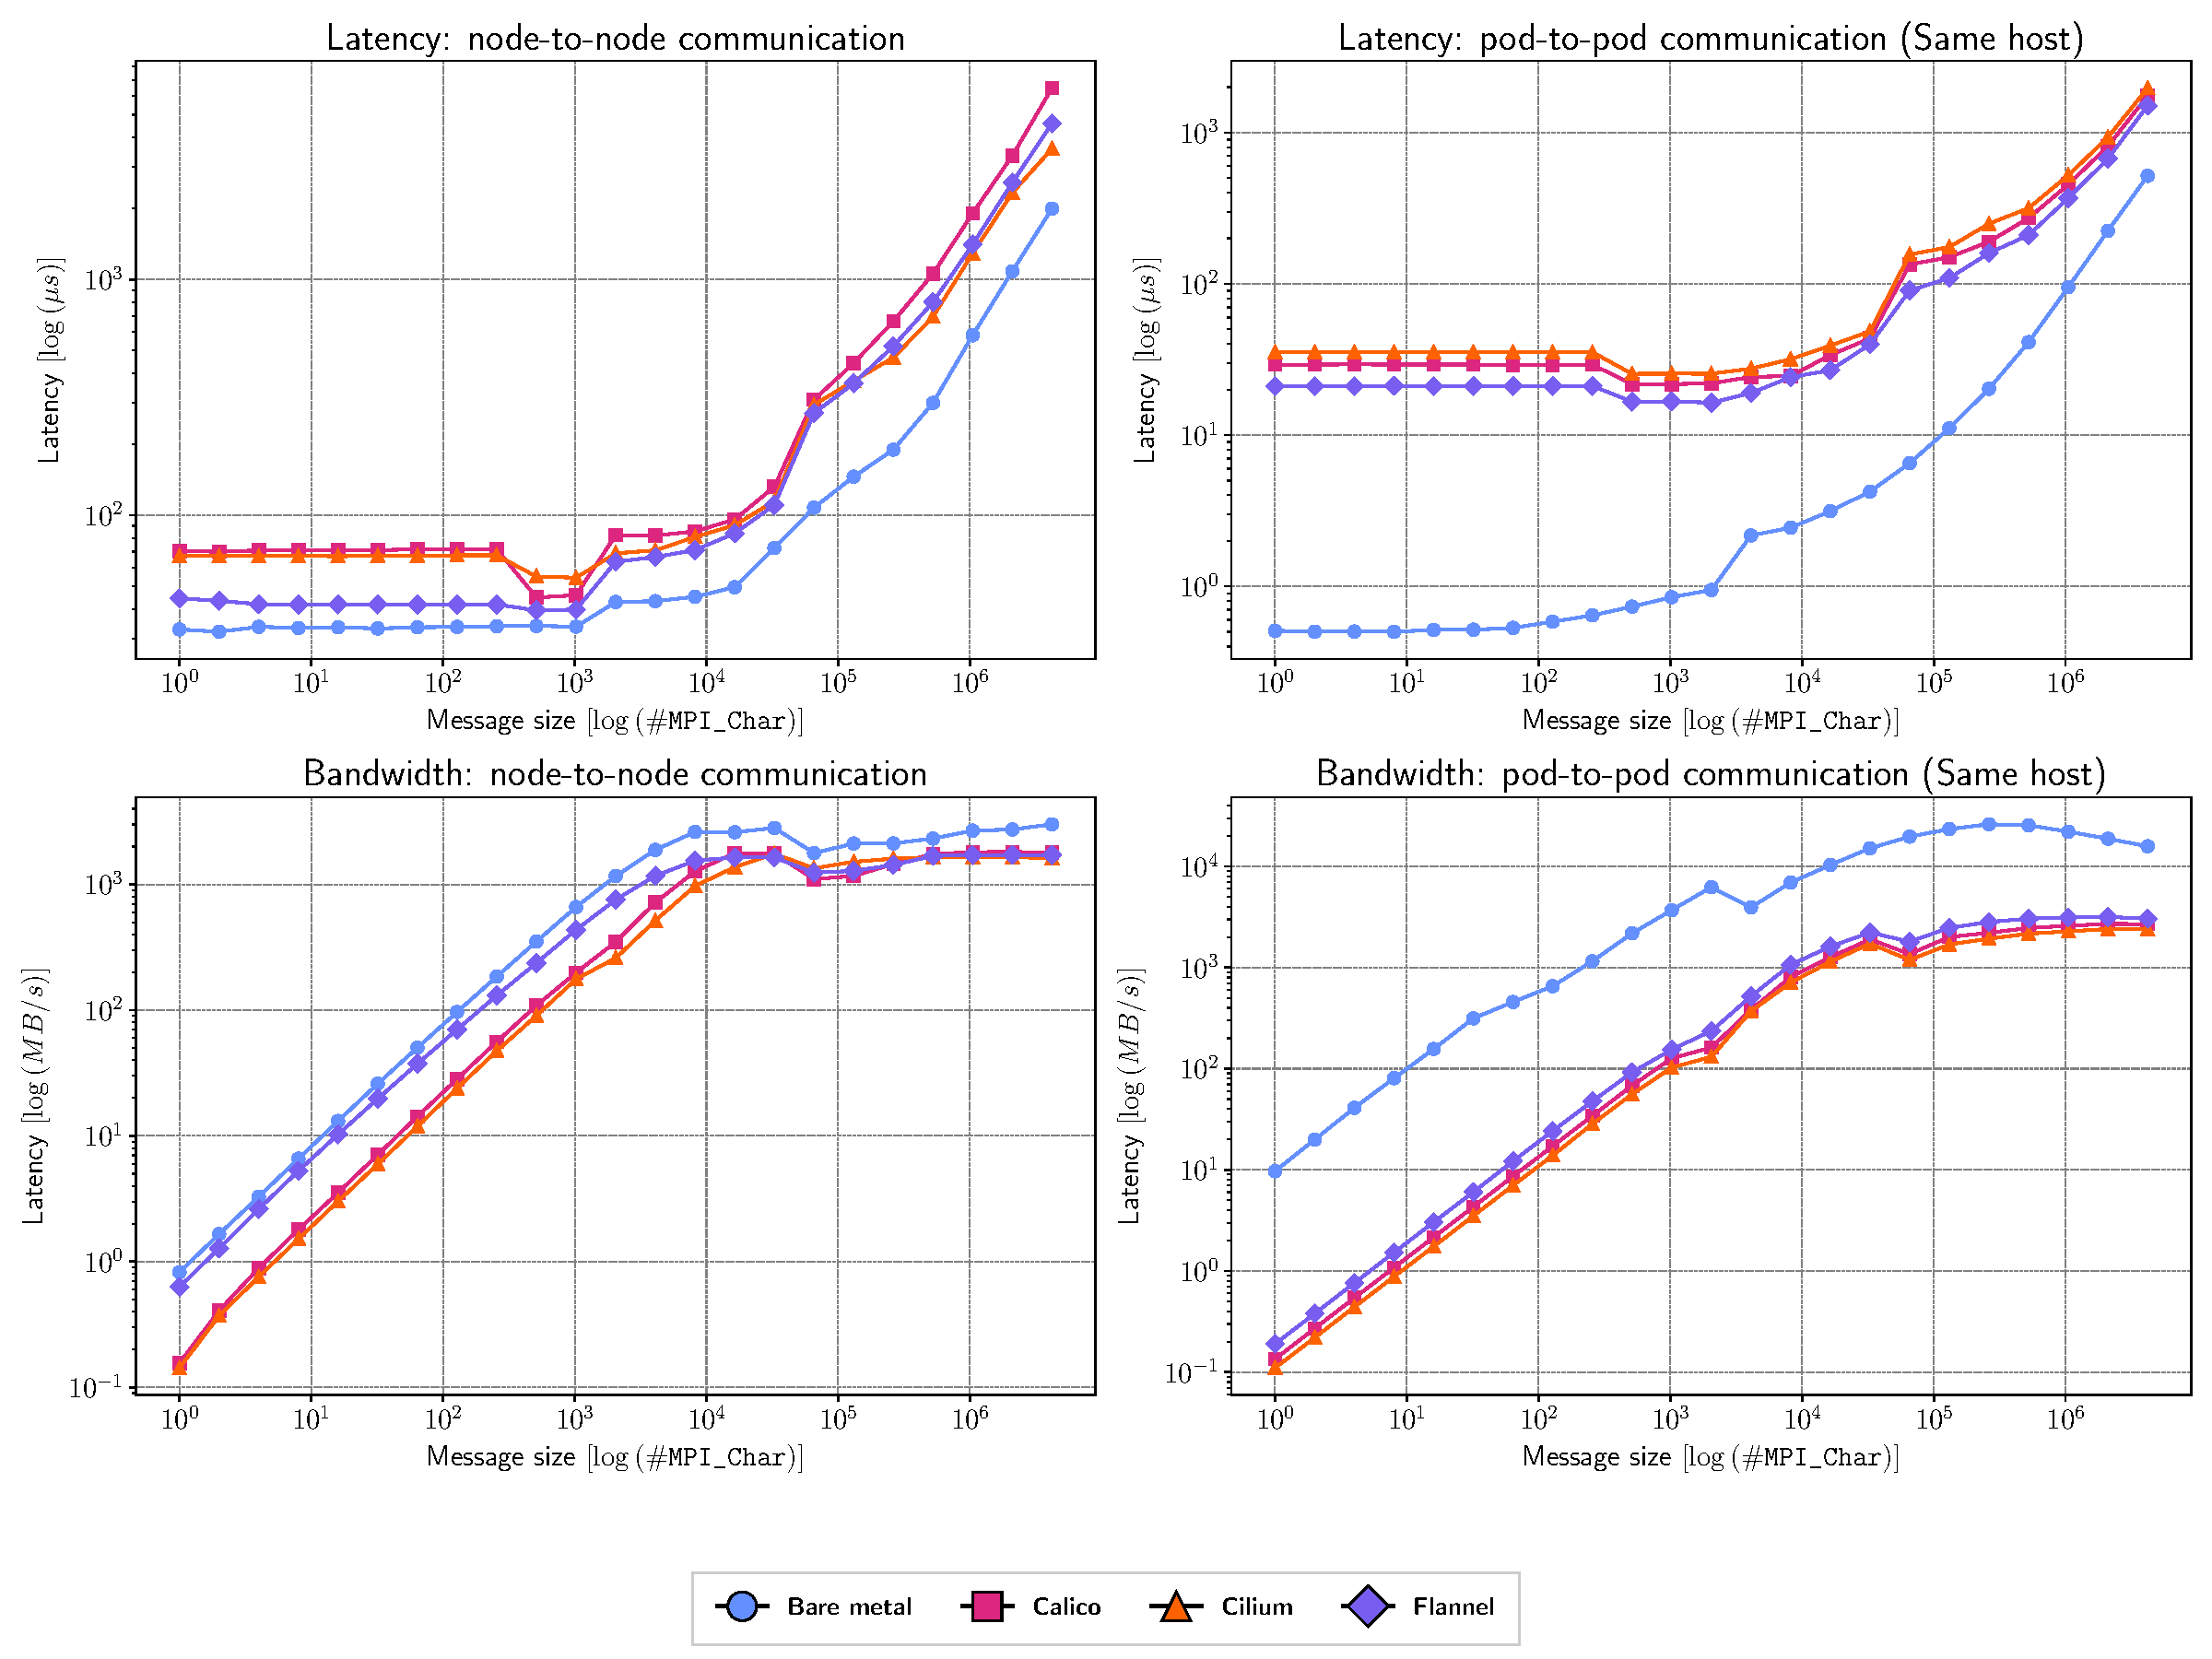
\includegraphics[width=0.8\textwidth]{img/abstract/summary-osu}
  \caption{Osu Micro-Benchmarks results. The top row shows the recorded latency
    (lower values are better) for different CNI and the baseline of a bare-metal
    calculation as a function of the MPI message size. The bottom row displays
    the bandwidth (higher values are better) for the same set of setups. The
    first column shows the result in node-to-node communication, and the second
    is in the pod-to-pod in the same node case compared with mpi processes on
    the same device as a bare metal reference. All benchmarks were executed 30
    times, and then the mean of all the measurements was considered.}
  \label{fig:summary-osu_en}
\end{figure}

Once we established that the cilium CNI plugin was the most attractive choice,
the next step was to evaluate the performance of the infrastructure on which the
code is running under a typical data science workload. The Dask Operator for
Kubernetes was utilized to do this. A net advantage of this choice is that it
can be reproduced in Slurm-based infrastructure. This possibility allows for
meaningful comparison between bare metal and Kubernetes tests. The Dask Operator
is a Kubernetes operator that manages Dask clusters. Removing the Kubernetes
abstraction, it is possible to spawn a Dask orchestrator that interacts with
SLURM to create a "cluster" object, a collection of "worker" objects. These
workers are the equivalent of worker pods in the Kubernetes infrastructure, each
of which is a separate process with a fixed amount of assigned resources. In
this test, we started with a single worker with one core and 3GB of RAM and
progressively increased the total number of workers to evaluate the weak
scalability.
Before delving into the results, it is essential to note that the hardware of
the Kubernetes cluster differs from that used in the bare metal evaluation due
to physical constraints. To enable a meaningful comparison, we applied a
normalization process. We assumed that running one application inside a
container \cite{deochake2023}   would not significantly impact the application's
performance. Therefore, all the values from the bare metal evaluation were
divided by a constant term. This term was defined as the factor by which the
1-core bare metal result must be divided to match the 1-core Kubernetes result.
Hence, the following results are not meant to be used to compare the performance
of the two infrastructures but to evaluate the scalability of the code in the
Kubernetes cluster and prove that the cloud-compliant implementation of the
cluster can scale as effectively as the bare metal one.
The following figure (Figure \ref{fig:summary-dask_en}) shows the results of the
evaluation of some of the most common operations performed on arrays:

\begin{figure}
  \centering
  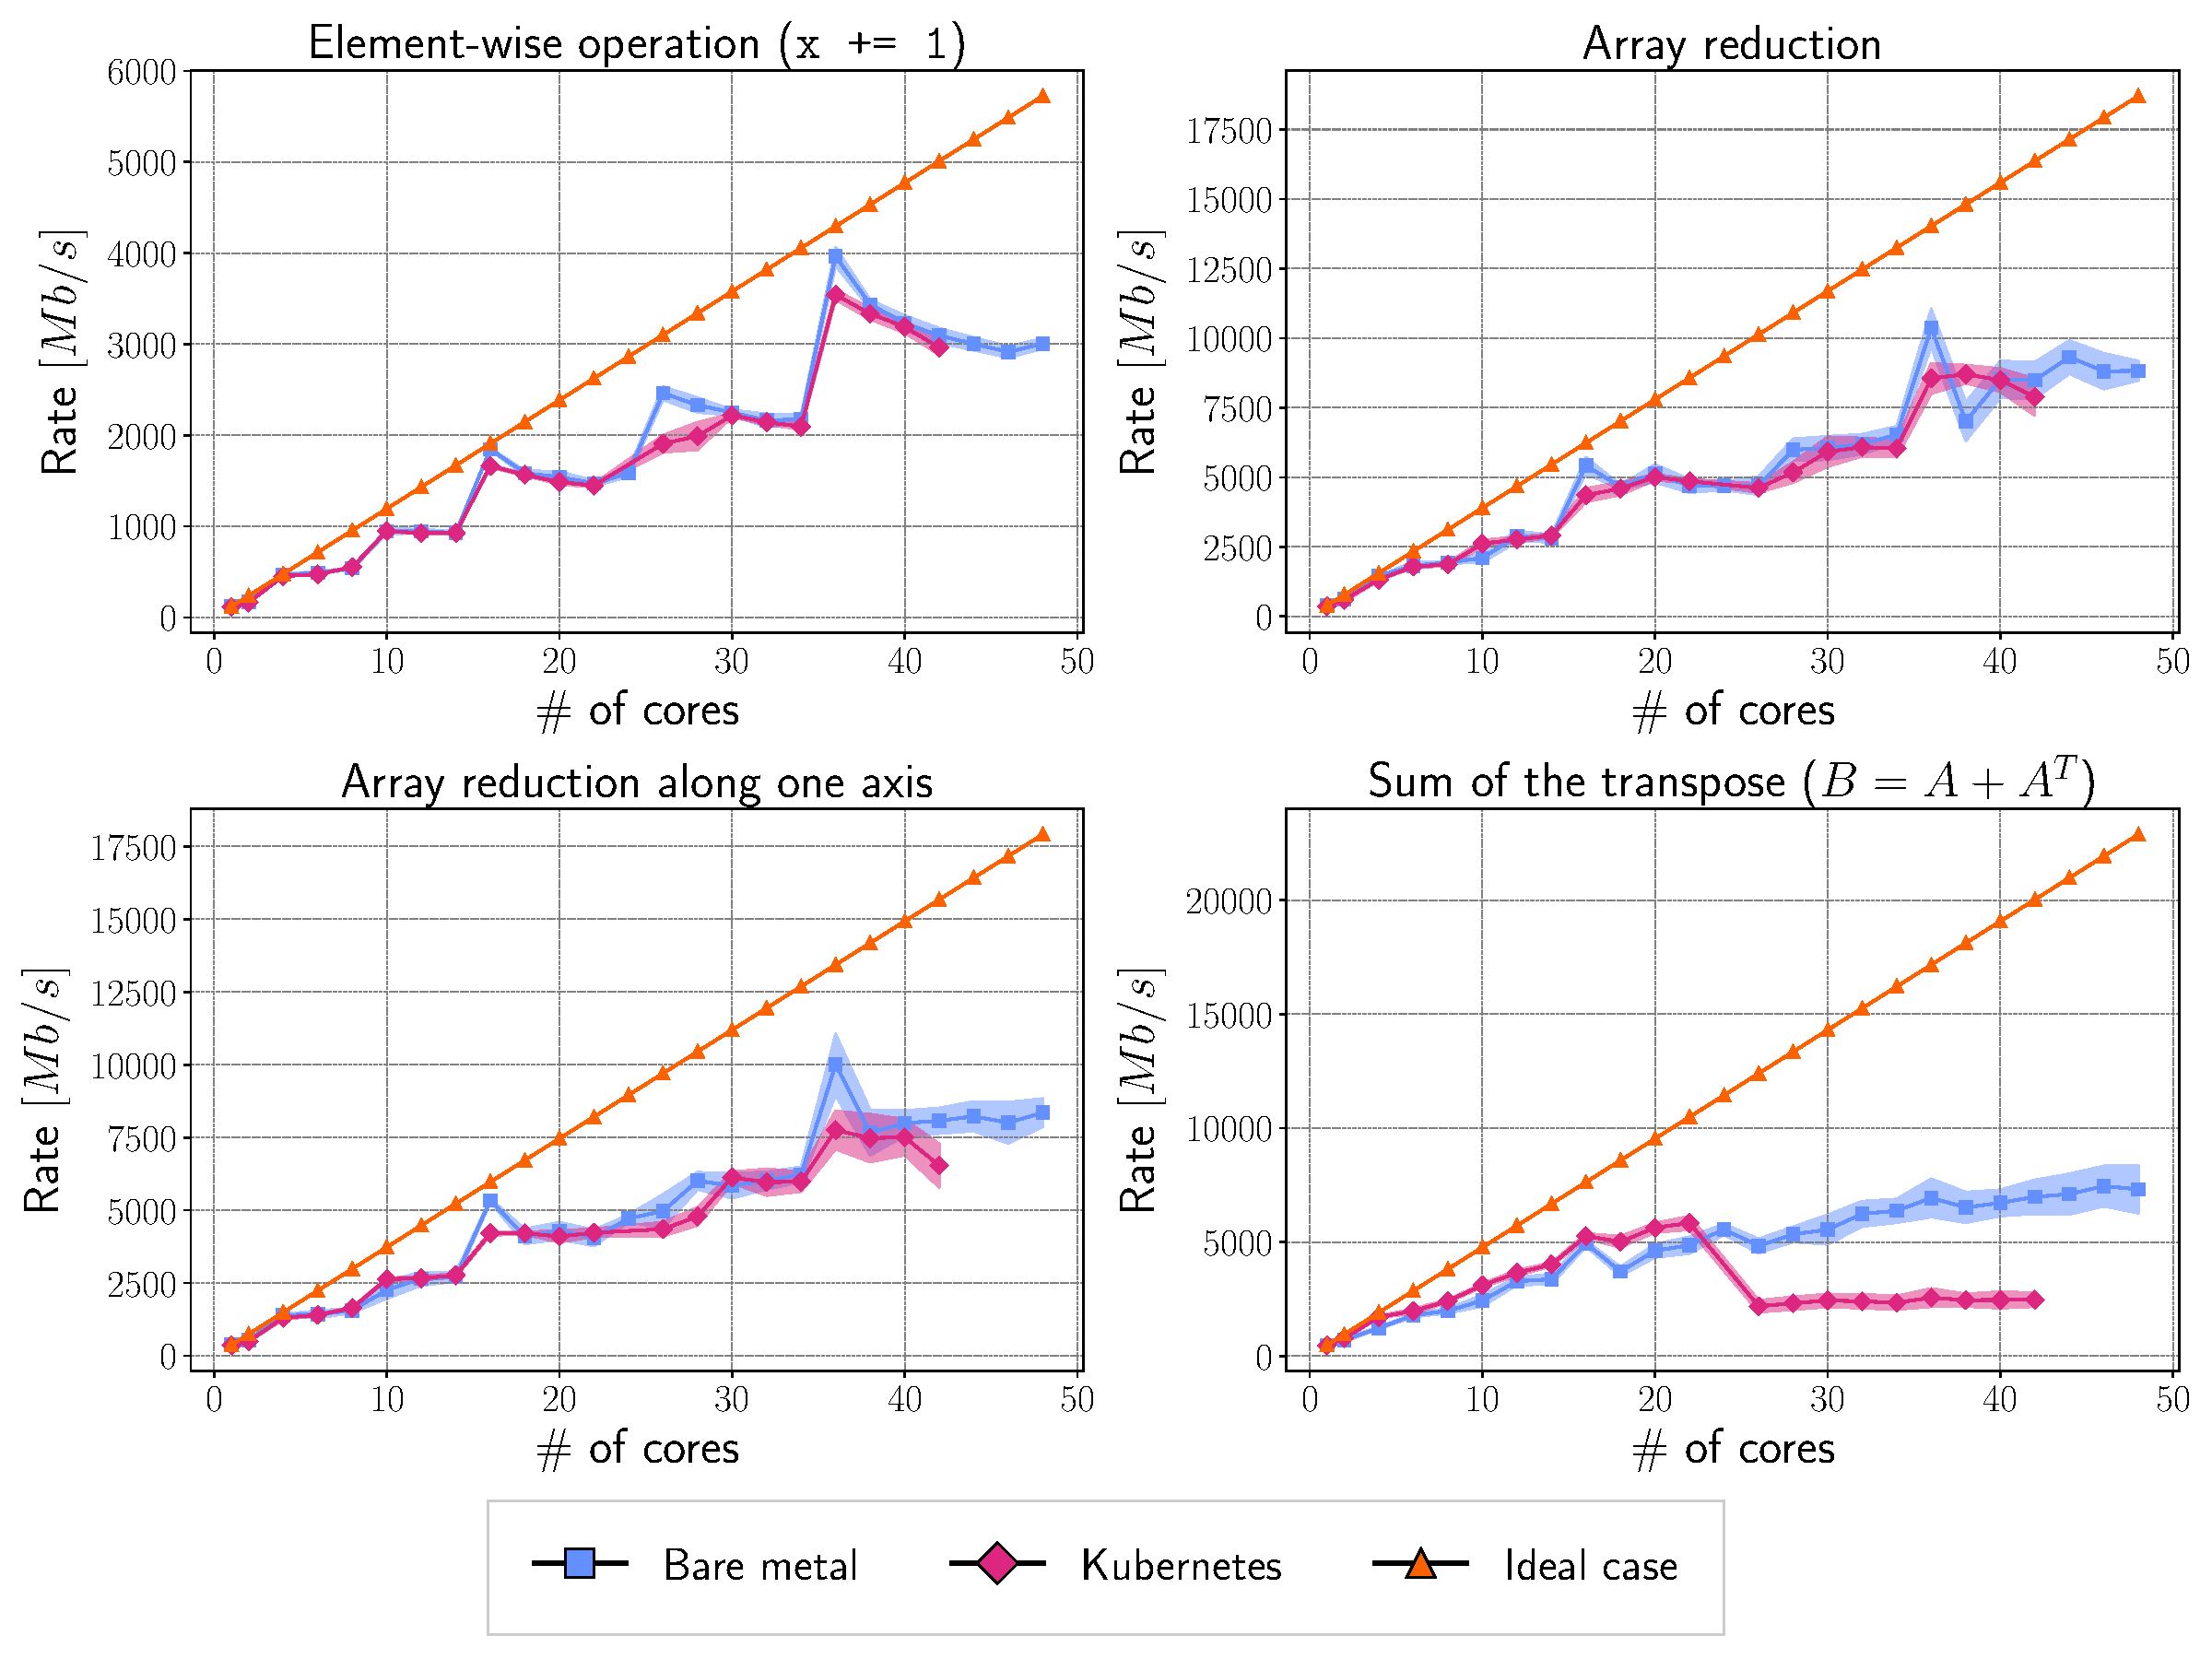
\includegraphics[width=0.8\textwidth]{img/abstract/summary-dask}
  \caption{Performance evaluation result of Dask for some of the most common operations applied to arrays. Each benchmark was run 30 times, and the average value was considered. These results, in particular, were obtained considering two-dimensional arrays.}
  \label{fig:summary-dask_en}
\end{figure}

From these very preliminary results, the code scalability in the proposed
Kubernetes setting is comparable to that obtained in the bare metal evaluation.
This is a promising result, as it shows that the proposed solution can fully
exploit the cluster resources, allowing the users to run parallel computation.
Moreover, it seems that using the Kubernetes cluster in our experiments leads to
better results (always considering the normalization processes). An explanation
could be that using the KUBECluster Dask object to create the cluster permits an
intelligent distribution of the workers on the nodes. For example, setting the
"PodAffinity" properly it is possible to ensure that the workers are scheduled
to fill an entire node before moving to the next one, reducing the communication
between the nodes as much as possible. In the bare metal evaluation in contrast,
the workers were created using the Dask SLURMCluster object, which allocates the
resources using an automatically generated script that uese the "sbatch" command
of the SLURM workload manager. In this second situation, the slurm manager is
responsible for distributing the workers on the nodes, and it is impossible to
establish any affinity between the workers and the nodes.As a result, workers
can be effectively distributed among all the nodes that make up the SLURM
partition of chioice. This distribution leads to a higher level of communication
between the nodes, potentially explaining the overall lower performance.

\section*{Conclusion}

In this work, we have analyzed the complexity of a cloud-ready HPC
infrastructure, individuating the key component that acts as a bottleneck when
trying to perform demanding tasks: networking.
After deploying the infrastructure and discussing its advantages, we focused on
networking. Here, we compared the latency and bandwidth performance of different
CNIs for Kubernetes infrastructure.
The main result is that when trying to parallelize the code using mpi, the
default Cilium installation, thanks to the ebpf dataplane, outperforms all other
solutions.
This advantage seems to become marginal when we leave mpi for more modern
parallelization frameworks, such as Dask, utilized by the data science
community.
However, Cillium is still incommensurably slower than the speed expected on an
ordinary HPC infrastructure where MPI can leverage the kernel verbs and an
Infiniband infrastructure.
To solve this problem, one possibility is to extend the test to the Mellanox CNI.
Furthermore, using Multus to deploy more than one CNI simultaneously could
enable the utilization of multiple network channels, potentially combining both
Ethernet and InfiniBand, thereby improving the overall network performance.
As a next step, we will add a user-friendly interface (JupyterHUB) that will
allow users to easily exploit all the advantages that the Kubernetes solution
entails, like standardization and greater code portability, auto-scaling of the
required resources, and in general, greater flexibility.
